\section{Introduction}
\label{sect:introduction}

Supersymmetry  (SUSY) \cite{Golfand:1971iw,Wess:1973kz,Wess:1974tw,Fayet1,Fayet2} is one of the most promising extensions of the 
standard model of the elementary particles (SM) which solves the 
quadratic divergences in the corrections to the mass of the Higgs boson from the fermions by introducing the new
bosons with proper couplings. The newly defined particles can fill the scales between the electroweak scale and 
the upper limit of the validity of SM and solve the  hierarchy problems, simultaneously. 
It introduces a new symmetry between the bosons and fermions and 
for every particle a sparticle is defined which is exactly the same, but differs in spin by 1/2. 
%Since the super particles are not discovered yet, the supersymmetry should be a broken symmetry. 
%Various mechanisms are introduced to break the symmetry softly without changing the other interesting features of the theory.
Extensive searches at the CERN LHC have pushed the mass of the colored SUSY particles much beyond the previous expectations \cite{Chatrchyan:2012sa,Chatrchyan:2012te,Chatrchyan:2012ira,Chatrchyan:2012qka,Chatrchyan:2011ek,Chatrchyan:2012ola,Chatrchyan:2012bba,Chatrchyan:2012mea,Chatrchyan:2013xna,Chatrchyan:2013xsw,Chatrchyan:2013wxa,Chatrchyan:2013fea}. %\cite{susyPhyRes}. 
Looking for the electroweak production of sparticles which has less hadronic activity and a comparable cross section is therefore well motivated.
% to not miss possible SUSY signals in a corner. 

A search for new physics using the full 2012 data is documented in this paper. 
The electroweak production of the SUSY particles with the leptonic final state was studied previously \cite{Khachatryan:2014qwa}.
In most of the SUSY models \cite{Martin:1997ns}, the third generation of the fermions are lighter than the two other generations. 
In the current analysis, due to the special role of the third generation of the sparticles, events with two $\tau$ leptons in the final state 
accompanied by a missing transverse energy (\MET) are considered. 
Tha ATLAS experiment has already published the results for a search for SUSY in di-$\tau$ final states \cite{Aad:2014yka}.
The two $\tau$ leptons can be generated in the cascade of the \sTau's or \PSGcpDo's:
\begin{linenomath}
\begin{equation}
p + p \rightarrow \PSGcpDo +\PSGcmDo ~~\mathrm{or}~~  p + p \rightarrow \sTau + \sTau,
\end{equation}
\end{linenomath}
when 
\begin{linenomath}
\begin{equation}
\PSGcpDo \rightarrow \sTau + \nu ~~\mathrm{or}~~  \PSGcpDo \rightarrow \sNu_{\tau} + \tau,
\end{equation}
\end{linenomath}
and 
\begin{linenomath}
\begin{equation}
\sTau \rightarrow \tau + \PSGczDo ~~\mathrm{or}~~  \sNu_{\tau} \rightarrow \nu + \PSGczDo.
\end{equation}
\end{linenomath}
The $\PSGczDo$ particle can not be detected and appears as \MET.
Figure \ref{fig:Productions} shows the main processes that can generate our favorite final state.
\begin{figure}[!Hhtb]
\centering
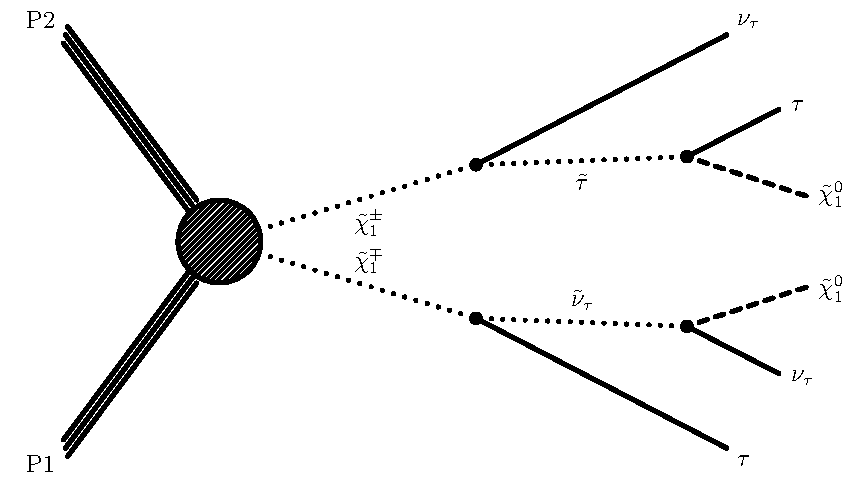
\includegraphics[width=0.49\textwidth]{Introductionfigs/TChipmSlepSnu.pdf}
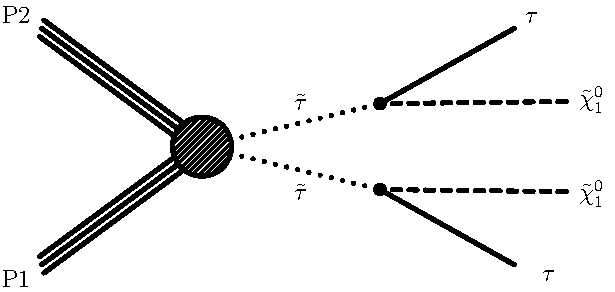
\includegraphics[width=0.49\textwidth]{Introductionfigs/TSlepSlep.pdf}
\caption{Schematic production of double $\tau$ from chargino pair and stau pair \cite{Khachatryan:2014qwa}. 
  In the figures $\ell$ and $\nu$ stand for $\tau$ and $\nu_{\tau}$, respevtively.}
\label{fig:Productions}
\end{figure}
%The production cross section of $\PSGcpDo\PSGcmDo$ is more than one order of magnitude higher than the
%production cross section of \sTau\sTau in the same mass of \sTau and \PSGcpDo.  
%For example for a 150 \GeV \sTau or \PSGcpDo, the cross section 
%of the pair production is 27 $fb$ and 1170 $fb$, respectively. Due to the higher cross section, 
Through this paper we focus on the $\PSGcpDo\PSGcmDo$ production. 
Although the search is sensitive to any high scale 
new physics with \MET, an R-parity conserving Simplified SUSY Model \cite{Alwall:2008ag,alves:sms} is used 
%to illustrate the performance of the method.
to interpret the results of the search.

%In the context of MSSM, supersymmetric objects are produced in pairs to conserve R-parity quantum number. Therefore in the production of charginos from proton-proton collisions, one may consider the following interaction $$pp\rightarrow\PSGcpDo\PSGcmDo\rightarrow\sTau^{+}\nu_\tau \sTau^{-}\nu_\tau\rightarrow\tau^{+}\PSGczDo\nu_\tau\tau^{-}\PSGczDo\nu_\tau\rightarrow\tau^{+}\tau^{-} + 2\,\PSGczDo + 2\,\nu_\tau.$$ In the detector, what can be observed are only 2 tau leptons plus missing transverse energy from the presence of neturinos and neutralinos in the final state.\\ 
The $\tau$ leptons decay leptonically ($e$ or $\mu$), in 35\% of the time, or decay via hadrons, which occurs in 65\% of the cases. Since there are two $\tau$ leptons in the final state, the probability of having $\PSGcpDo\PSGcmDo \rightarrow \hadtau+e/\mu+\MET$ is about 46\%, while the probability for $\PSGcpDo\PSGcmDo \rightarrow \hadtau+\hadtau+\MET$ to occur is about 42\%. Hereafter, final states containing a lepton are referred to as $\leptonTau$ channel and those events where the two $\tau$'s decay via hadrons are referred to as $\tauTau$ channel. 
%The selection cuts to enhance $\tauTau$ events will be discussed in Section~\ref{sect:tauTauCuts}. The list of cuts to select $\leptonTau$ events can be found in Section~\ref{sect:leptonTauCuts}.\\     

The search variable is the stransverse mass (\mttwo, section \ref{sect:mt2def}) 
which is the natural extension of the known transverse mass (\mt) to a case 
when two massive particles with equal mass are created in pairs and decay 
%via a chain of jets and leptons 
to two invisible particles accompanied by jets and leptons, similar to our case.
%In the case of R-parity conserving SUSY, the Lightest Supersymmetric Particle (LSP), \PSGczDo in our scenario, 
%escapes  detection and appears as \MET.

The current paper is organized as follows, after introduction in the next section the CMS experiment  
and objects used in this analysis are introduced. The \mttwo variable is introduced in sections \ref{sect:mt2def}. 
The events selections for different channels are shown in sections \ref{sect:tauTauCuts} and \ref{sect:eleTauCuts}. 
A detailed study of the SM backgrounds is presented in section \ref{sect:bkgLepTau}. Section \ref{sect:sys} 
is devoted to evaluation of the systematic uncertainties. The final numbers and their statistical interpretation is presented in 
section \ref{sect:stat} and finally section \ref{sect:conclusion} concludes the paper.





